\chapter{Data Understanding and Preparation}
\label{ch:capitolo1}

The dataset \textit{train.csv} contains 16431 titles of different forms of visual entertainment that have been rated on IMDb, 
an online database of information related to films, television series etc. 
Each record is described by 23 attributes, either discrete or continuous.

\section{Discrete Attributes}
Table~\ref{tab:attributes} shows the discrete attributes of the dataset,
their types and a brief description of each attribute.
\begin{table}[h]
\centering
\begin{tabular}{lll}
\toprule
\textbf{Attribute} & \textbf{Type} & \textbf{Description} \\
\midrule
\texttt{originalTitle} & Categorical & Title in its original language \\
\texttt{rating} & Ordinal & IMDB title rating class, from \texttt{(0,1]} to \texttt{(9,10]} \\
\texttt{worstRating} & Ordinal & Worst title rating \\
\texttt{bestRating} & Ordinal & Best title rating \\
\texttt{titleType} & Categorical & The format of the title \\
\texttt{canHaveEpisodes} & Binary & Whether the title can have episodes: \texttt{True}/\texttt{False} \\
\texttt{isRatable} & Binary & Whether the title can be rated: \texttt{True}/\texttt{False} \\
\texttt{isAdult} & Binary & Whether the title is adult content: \texttt{0} (non-adult), \texttt{1} (adult) \\
\texttt{countryOfOrigin} & List & Countries where the title was produced \\
\texttt{genres} & List & Genre(s) associated with the title (up to 3) \\
\bottomrule
\end{tabular}
\caption{Description of discrete attributes}
\label{tab:attributes}
\end{table}
\vspace{-1em}
\subsection{Merging and Removal of Discrete Attributes}\label{subsec:var_elim_discrete}
The following discrete attributes were removed from the dataset:
\begin{itemize}
    \item \texttt{originalTitle} was removed because it is not relevant for the analysis;
    \item the \texttt{isRatable} variable was removed because all the titles in the dataset are ratable;
    \item \texttt{worstRating} and \texttt{bestRating} attributes were removed because they assume the same values for all records (1 and 10 respectively).
\end{itemize}

Additionally, the \texttt{isAdult} attribute is highly correlated with the presence or absence of
\textit{Adult} in \texttt{genre} (16 records differ in the train set, 1 in the test set), so the two were
merged with a logical OR operation. This is not true for the \textit{short} type in \texttt{titleType}, with
491 records having different values from the obtained feature. For this reason, the two were kept separate.



\subsection{Discrete Attributes Analysis}
This paragraph provides an overview of the discrete attributes in the dataset, focusing on their distributions and statistics.
Figures~\ref{fig:titleType_distrib} and~\ref{fig:rating_distrib} show bar plots of \texttt{titleType} and \texttt{rating} attributes, respectively.\\
Figure~\ref{fig:titleType_distrib} shows that the classes of the \texttt{titleType} attribute are imbalanced, with \textit{movie} being the most frequent class (5535 records).
It was observed that the class \textit{tvShort} is the least frequent in the dataset, with only 40 records (around 0.24\% of the dataset). Because of this, these rows were discarded from the dataset, as they were considered irrelevant for the analysis.
The decision was not repeated for \textit{tvSpecial} and \textit{tvMiniSeries}, as they cover slightly more than 1\% of the dataset each (166, 1.01\% and 224, 1.36\%, respectively).
\begin{figure}[H]
    \centering
    % First subfigure
    \begin{subfigure}{0.45\textwidth}
        \centering
        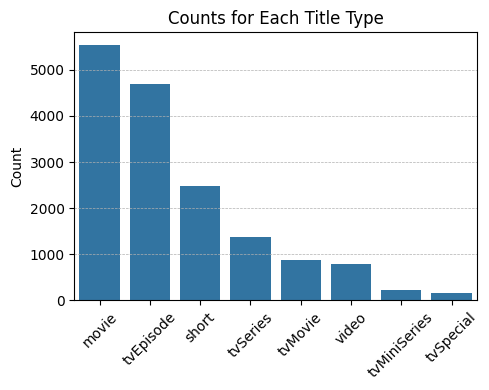
\includegraphics[width=0.98\textwidth]{plots/types_count.png}     %se teniamo 0.65 ci sta sotto la tabella delle continuous
        \caption{Distribution of \texttt{titleType}}
        \captionsetup{width=0.9\linewidth, justification=centering}
        \label{fig:titleType_distrib}
    \end{subfigure}
    \begin{subfigure}{0.47\textwidth}
        \centering
        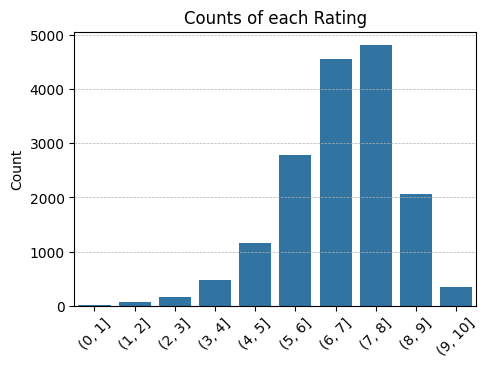
\includegraphics[width=0.98\textwidth]{plots/rating_distrib.png}     %se teniamo 0.65 ci sta sotto la tabella delle continuous
        \caption{Distribution of \texttt{rating}}
        \captionsetup{width=0.9\linewidth, justification=centering}
        \label{fig:rating_distrib}
    \end{subfigure}
    \captionsetup{justification=centering}
    \caption{Distribution of the \texttt{titleType} and \texttt{rating} attributes}
    \label{fig:distrib_categorical}
\end{figure}

As shown in figure~\ref{fig:rating_distrib}, the \texttt{rating} attribute roughly follows a normal distribution, with a slightly asymmetric peak:
a significant number of titles falls within the (6,7] and (7, 8] ranges (4565 and 4822 titles, respectively) while only a total amount of 67 titles falls within (0,1] and (1,2].
% The overall distribution resembles a normal distribution, with a slightly asymmetric peak.


\subsection{Encoding and Transformation of Categorical Attributes}
The attribute \texttt{rating} was transformed by taking the upper bound of each rating
interval's string representation. This approach was chosen because the minimum rating is 1, meaning the
lowest interval corresponds only to ratings of 1. For consistency, the same transformation was applied
to all other intervals.
Multi-label one-hot encoding was applied to the \texttt{genres} column. 
Each unique genre was represented as a binary feature, allowing records that belong to multiple genres simultaneously to maintain this information; this generated 28 new features.
Depending on the task, some were often discarded to avoid overfitting or to reduce the number of features.
Rows with no genres were assigned a vector of all zeros, indicating the absence of any genres.\\

% After that, multi-label one-hot encoding was applied to the
% \texttt{genres} column; each unique genre was represented as a binary feature, 
% allowing records that belong to multiple genres simultaneously to maintain this information.
% \vspace{1em}
The attribute \texttt{countryOfOrigin} was represented by grouping the countries by continent.
The following variables have been created: 
\begin{multicols}{2}
    \begin{itemize}
        \item \texttt{countryOfOrigin\_freq\_enc}\\ 
        (frequency encoding of the original list);
        \item \texttt{countryOfOrigin\_AF} (Africa);
        \item \texttt{countryOfOrigin\_AS} (Asia);
        \item \texttt{countryOfOrigin\_EU} (Europe);
        \item \texttt{countryOfOrigin\_NA} (North America);
        \item \texttt{countryOfOrigin\_SA} (South America);
        \item \texttt{countryOfOrigin\_OC} (Oceania);
        \item \texttt{countryOfOrigin\_UNK} (Unknown country).
    \end{itemize}
\end{multicols}


For each record, the first six features provide the number of countries for each continent.
The \texttt{countryOfOrigin\_UNK} variable counts the number of countries that are not recognized as
belonging to a continent for that record.
% Each of the first six features provides the number of countries in the corresponding continent.\\
% \texttt{countryOfOrigin\_UNK} is used to represent the strings that are not categorized as being part of a
% continent, by counting the strings that are not recognized.
Additionally, \texttt{countryOfOrigin\_freq\_enc} provides the frequency encoding of the original list of countries as a whole, 
showing how frequently a specific combination of countries appears across the entire dataset.
% In summary, the original attribute is represented by the seven features regarding
% the continents, plus 1 representing the frequency encoding.
These transformations allow to keep most of the original information, while limiting the number of new features.




\section{Continuous Attributes}
Table~\ref{tab:numerical_attributes} shows the continuous attributes of the dataset, their type and
a brief description.
\vspace{1em}
\begin{table}[H]
    \centering
    \begin{tabular}{lll}
        \toprule
        \textbf{Attribute} & \textbf{Type} & \textbf{Description} \\
        \midrule
        \texttt{runtimeMinutes} & Integer & Runtime of the title expressed in minutes \\
        \texttt{startYear} & Integer & Release/start year of a title \\
        \texttt{endYear} & Integer & TV Series end year \\
        \texttt{awardWins} & Integer & Number of awards the title won \\
        \texttt{numVotes} & Integer & Number of votes the title has received \\
        \texttt{totalImages} & Integer & Number of images on the IMDb title page \\
        \texttt{totalVideos} & Integer & Number of videos on the IMDb title page \\
        \texttt{totalCredits} & Integer & Number of credits for the title \\
        \texttt{criticReviewsTotal} & Integer & Total number of critic reviews \\
        \texttt{awardNominationsExcludeWins} & Integer & Number of award nominations excluding wins \\
        \texttt{numRegions} & Integer & Number of regions for this version of the title \\
        \texttt{userReviewsTotal} & Integer & Number of user reviews \\
        \texttt{ratingCount} & Integer & Total number of user ratings for the title \\
        \bottomrule
    \end{tabular}
    \caption{Description of continuous attributes}
    \label{tab:numerical_attributes}
\end{table}

\subsection{Removal and Merging of Continuous Attributes}\label{sec:var_elim_creation}
The plot in figure~\ref{fig:correlation_matrix} is a Pearson's correlation matrix that takes into
account the continuous attributes of the dataset.
The matrix shows that \texttt{ratingCount} and \texttt{numVotes} are perfectly correlated;
for their redundancy, \texttt{ratingCount} was discarded.\\
\begin{figure}[H]
    \centering
    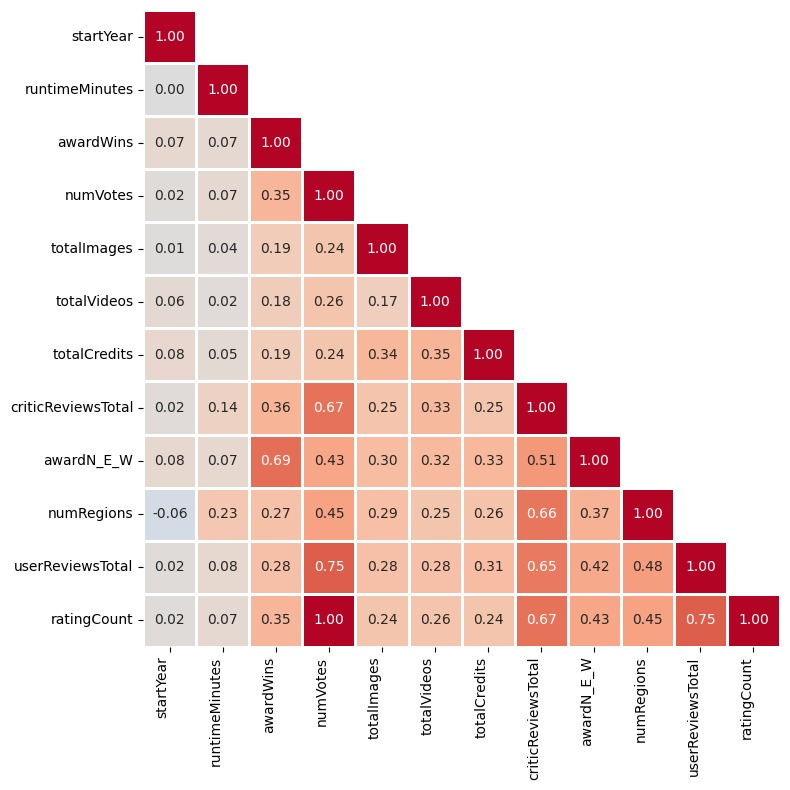
\includegraphics[width=0.50\textwidth]{plots/correlation_matrix.png}
    \captionof{figure}{Correlation matrix}
    \label{fig:correlation_matrix}
\end{figure}

% \begin{wrapfigure}{r}{0.55\textwidth}
%     \centering
%     \captionsetup{justification=raggedleft, width=1\linewidth}
%     \caption{Correlation matrix}
%     \label{fig:correlation_matrix}
%     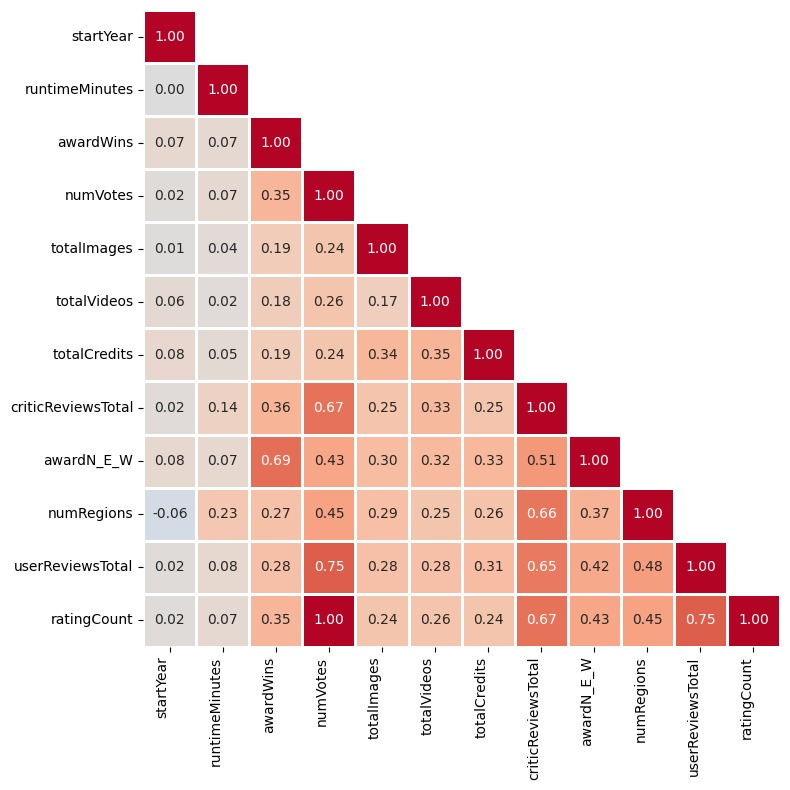
\includegraphics[width=0.9\linewidth]{plots/correlation_matrix.png}
% \end{wrapfigure}
The attributes \texttt{awardNominationsExcludeWins} and \texttt{awardWins} were combined into 
\texttt{totalNominations}, due to their strong semantic similarity and high correlation (0.69).
The new feature represents the sum of the two original attributes. This transformation also helps
mitigate the impact of their heavy right skew (shown in figure\ref{fig:sub1}), resulting in a more meaningful and interpretable feature.
Similarly, the \texttt{totalVideos} and \texttt{totalImages} attributes were combined into a single
feature, i.e. \texttt{totalMedia}, representing the total number of media items associated with a title.
Although the original attributes are not highly correlated, both exhibit skewed distributions (as in figure\ref{fig:sub2}), \texttt{totalVideos} in particular.
Due to this, and to their similar semantic meaning, they were merged to form a more consolidated and
interpretable feature.

\begin{figure}[H]
    \centering
    % First subfigure
    \begin{subfigure}{0.41\textwidth}
        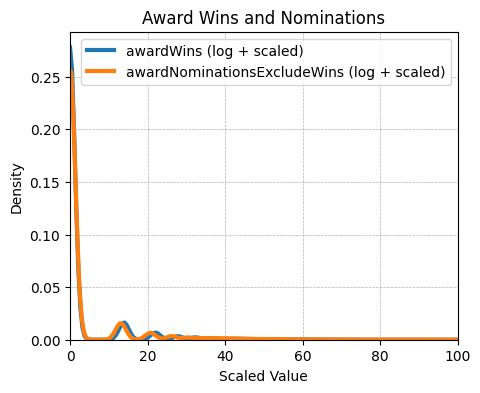
\includegraphics[width=\textwidth]{plots/nominations_distrib.png}
        \captionsetup{width=0.9\linewidth, justification=centering}
        \caption{Kernel Density Estimation of \texttt{awardWins} and \texttt{awardNominationsExcludeWins}}
        \label{fig:sub1}
    \end{subfigure}
    \begin{subfigure}{0.41\textwidth}
        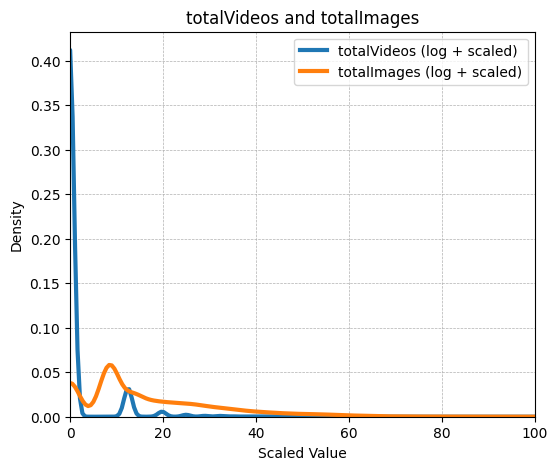
\includegraphics[width=\textwidth]{plots/totalVideos_Images_distrib.png}
        \captionsetup{width=0.9\linewidth, justification=centering}
        \caption{Kernel Density Estimation of \texttt{totalVideos} and \texttt{totalImages}}
        \label{fig:sub2}
    \end{subfigure}
    \captionsetup{justification=centering}
    \caption{Distribution of the attributes that form the \texttt{totalNominations} and \texttt{totalMedia} features}
    \label{fig:distrib}
\end{figure}

Although \texttt{criticReviewsTotal} and \texttt{userReviewsTotal} also have a relatively high correlation (0.65), as well as a right-skewed distribution, 
it was decided that the two attributes should be kept separate because of their relevance in meaning. It is also worth noting that the two have high correlations with 
\texttt{numVotes} (0.67 and 0.75 respectively), but they were all kept because of the difference between votes and reviews.



\section{Data Quality}\label{sec:data_quality}
Next, a proper evaluation of the observed data was conducted in preparation for the analysis.
Once having checked that there are no duplicates and no incomplete rows in the dataset,
attention was given at identifying missing values and outliers.

% parte che ci sembrava importante per far vedere che ce ne siamo accorti
% \subsection{Syntactic Inconsistencies} 
% Even though \texttt{awardWins} was the only feature having missing values marked with \texttt{NaN}, 
% it has been noticed that there were missing values also in other columns - \texttt{endYear}, \texttt{runtimeMinutes} and \texttt{genres} -
% marked with the string "\textbackslash N" instead.
% To avoid this inconsistency those values have been replaced with \texttt{NaN}.


\subsection{Missing Values}\label{sec:missing_values}
% The missing values in the above-mentioned attributes were handled as follows:
The following attributes were found to have missing values\footnote{missing values were marked as \texttt{NaN}
only in \texttt{awardWins}; in the other listed columns \texttt{"\textbackslash N"} was used, so it was then converted to \texttt{NaN}}:
\begin{itemize}
    \item \texttt{endYear}: it is the feature with the highest number of \texttt{NaN} values (15617; about 95\%).
    Although the feature is only relevant for \textit{TVSeries} and \textit{TVMiniSeries} titles, it still
    had approximately 50\% missing values within those categories, limiting its usefulness even in the
    appropriate context. For this reason, the feature was discarded.
    \vspace{1em}
    
    \item \texttt{runtimeMinutes}: this attribute has 4,852 missing values (29.5\%). Two imputation strategies were employed, both based on random sampling within the interquartile range. 
    The first used \texttt{titleType} to define the range, while the other imputed values based off of the attribute's distribution alone. 
    The choice of which of the two strategies to use depends on the specific task, and will be specified in the corresponding sections.
    
    \item \texttt{awardWins}: this feature has 2618 \texttt{NaN} values (about 16\%).
    Since the mode associated with this variable is 0, it has been decided to substitute the missing
    values with 0.

    \item \texttt{genres}: it has 382 missing values (2.3\%). Having dealt this variable with a
    multi-label one-hot encoding process (as has been described in the \textit{Encoding and Transformation of categorical attributes}
    section), a vector of all zeros is assigned to records with missing genres values.
\end{itemize}



\subsection{Semantic Inconsistencies, Feature Transformations and Outlier detection}
While analyzing the dataset, it was observed that the \textit{Videogame} type of the \texttt{titleType} attribute (259 records - around 1.58\% of the dataset) 
was not consistent with the other values of the same feature, being \textit{Videogame} a fundamentally different type.
These rows also generated problems for some of the other attributes, such as \texttt{runtimeMinutes}, resulting in most values being missing and difficult to impute. 
Because of this, the samples were removed from the dataset. \\


Some features showed a heavy right-skewed distribution, with typical traits of Power-Law Distributions. Their Kernel Density Estimations are shown in figure~\ref{fig:left_skewed}.

\begin{figure}[H]
    \centering
    \begin{subfigure}{0.48\textwidth}
        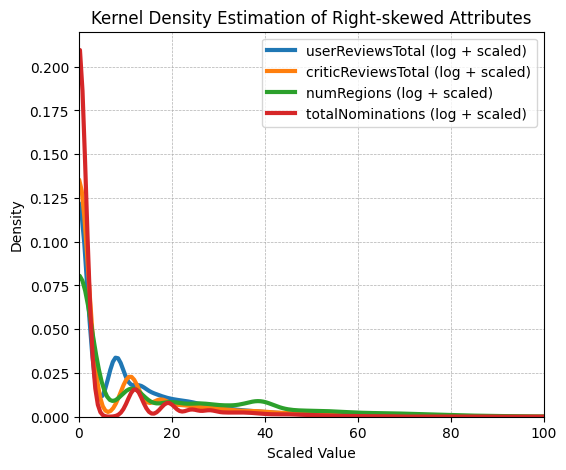
\includegraphics[width=\textwidth]{plots/left_skew_distribs.png}
        \captionsetup{width=0.9\linewidth, justification=centering}
        \caption{KDE of right-skewed attributes}
        \label{fig:sub1_KDE_left_skew}
    \end{subfigure}
    \begin{subfigure}{0.48\textwidth}
        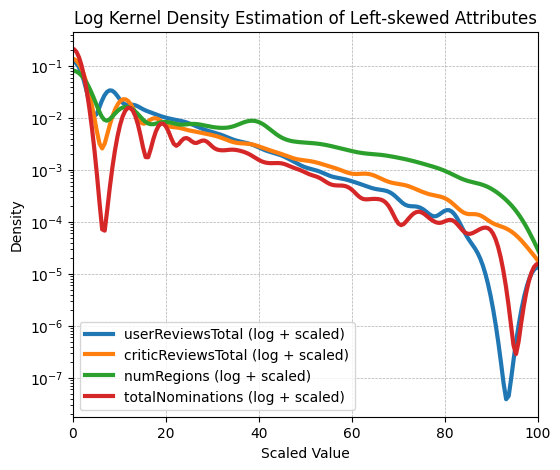
\includegraphics[width=\textwidth]{plots/left_skew_distribs_log.png}
        \captionsetup{width=0.9\linewidth, justification=centering}
        \caption{KDE of right-skewed attributes with log density}
        \label{fig:sub2_KDE_left_skew}
    \end{subfigure}
    \caption{Kernel Density Estimation of the right-skewed attributes}
    \label{fig:left_skewed}
\end{figure}

The decay of these features is exponential in linear space (~\ref{fig:sub1_KDE_left_skew}), while in logarithmic space there is a decline that can be approximated to a linear trend (~\ref{fig:sub2_KDE_left_skew}). 
For this reason, when needed, a log-transformation was applied to these attributes to reduce the skewness and make
them more suitable for some specific analysis.
Because of right-skewness (without a power-law distribution), other attributes were also log-transformed:
\begin{itemize}
    \item \texttt{numVotes};
    \item \texttt{totalCredits};
    \item \texttt{totalMedia}.
\end{itemize}



\begin{wrapfigure}{r}{0.45\textwidth}
    \centering
    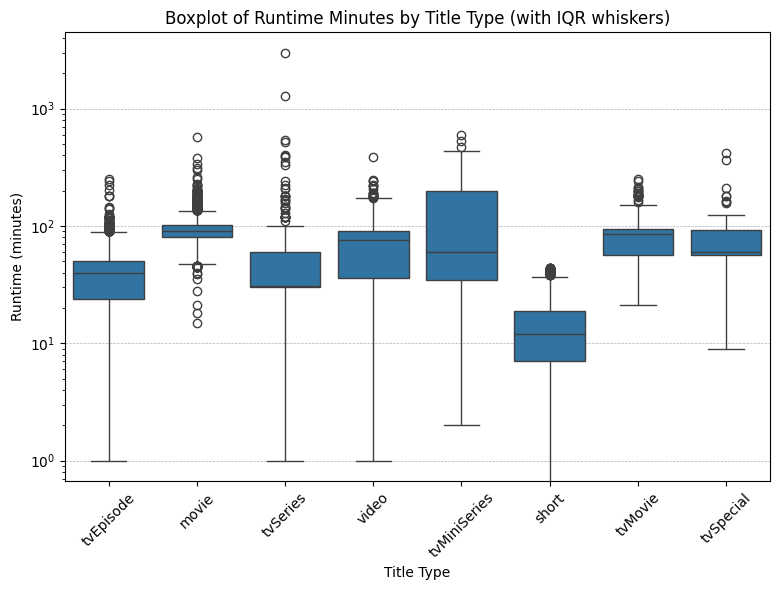
\includegraphics[width=1\linewidth]{plots/outliers.png}
    \captionsetup{width=0.9\linewidth, justification=raggedleft}
    \caption{Boxplot of the \texttt{runtimeMinutes} attribute for each \texttt{titleType}}
    \label{fig:outliers}
\end{wrapfigure}
Regarding outliers, \texttt{runtimeMinutes} was the most problematic feature.
Similarly to missing values imputation (~\ref{sec:missing_values}),
outlier detection was performed using two different strategies:
% Figure~\ref{fig:runtimeMinutes_boxplot} shows the first approach, which computes outliers on each \texttt{titleType} separately.
the first approach computes outliers on each \texttt{titleType} separately,
while the second is based on the distribution of the \texttt{runtimeMinutes} attribute alone.
Figure~\ref{fig:outliers} reports an analysis of the feature through the IQR method separately on each type.
The boxplots show that there are samples that have been misreported, with runtimes of over 1000 minutes for \textit{tvSeries}.
% the same can be observed on the second plot on the \textit{Has episodes} box plot.
This might be because of an inconsistency with the understanding of the meaning of the attribute, and in those cases it might be possible that
the value refers to the total runtime of the series, rather than the runtime of a single episode.
% Another interesting observation regards the presence of records with a runtime of 0 minutes for the \textit{short} type. This was present in just 1 record, and it was removed from the dataset because it was considered a mistake, although it was not considered an outlier.\\
Another interesting observation regards the presence of a record with a runtime of 0 minutes for the \textit{short} type;
% although it was not considered an outlier by the first method,
the record was removed because it was regarded as an erroneous sample.
Other than this sample, other outliers were not removed from the dataset by default. Instead, a case-by-case approach was adopted,
testing each task and analysis both with and without the outliers. Notably, in every case, better results were obtained when outliers were excluded.